%  --------------------------------------------------  Lectures by Mirafra -------------------------------------------
The following tutorials explain and demonstrate all
steps in the process of transforming C, C++ and SystemC code to an RTL implementation
using High-Level Synthesis. These show how to create an initial RTL implementation
and then transform it into both a low-area and high-throughput implementation by
using optimization directives without changing the C code. 

\begin{highlight}
Reference for this sections: Vivado Design Suite Tutorial High-Level Synthesis UG871
\end{highlight}


\section{High-Level Synthesis Introduction}
This tutorial introduces Vivado High-Level Synthesis (HLS). The primary
tasks for performing High-Level Synthesis using both the Graphical User Interface (GUI) and
Tcl environments are demonstrated.

\subsection{Lab 1: Creating a High-Level Synthesis Project}
This lab explains how to set up a High-Level Synthesis (HLS) project and perform all the major steps in the HLS design flow:

\begin{enumerate}[label=Step \arabic*:]
    \item Creating a New Project: 
    \begin{enumerate}
        \item Open HLS GUI
        \item Enter project details (Name, Location)
        \item Add source files
        \item Add test bench files
        \item Generate Solution (specify hardware details \eg clock period, FPGA part, clock uncertainty)
    \end{enumerate}    
    \item Validate the C code (C Validation or C Simulation):\\
    Aim of this step is to confirm that the C code is correct. This process is also called {\bf C Validation or C Simulation.}
    \item High-Level Synthesis:\\ Synthesize the C design into an RTL design and review the synthesis report.
    \item RTL Verification:\\ High-Level Synthesis can re-use the C test bench to verify the RTL using simulation.
    \item IP Creation:\\ To package the design as an IP block for
    use with other tools in the Vivado Design Suite.
\end{enumerate}


\subsubsection{HLS Graphical User Interface (GUI)} 
Regions in the Graphical User Interface (GUI) and their functions are:
\begin{figure}[H]
    \begin{center}
        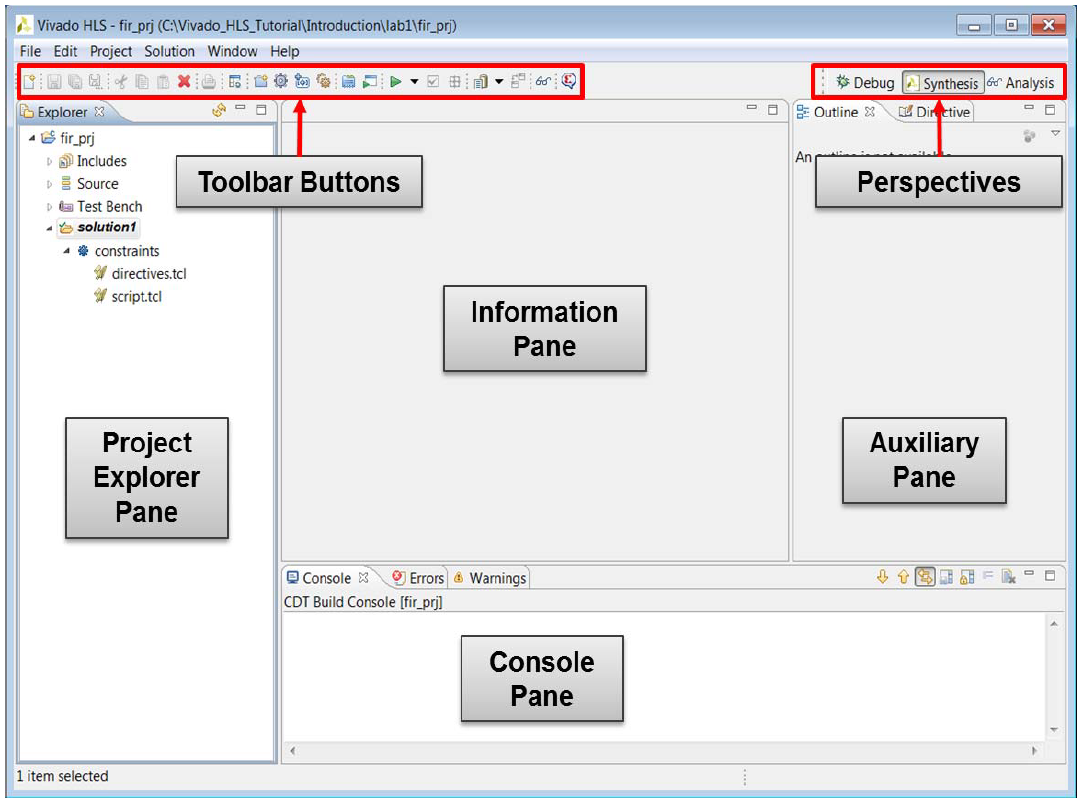
\includegraphics[width=0.8\textwidth]{images/panes.png}
        \caption{Vivado HLS Graphical User Interface}
        \label{panes}
    \end{center}
  \end{figure}

\begin{description}
    \item[Explorer Pane] Shows the project hierarchy.
    \item[Information Pane] Shows the contents of any files opened from the Explorer pane along with report files.
    \item[Auxiliary Pane] Cross-links with the Information pane.
    \item[Console Pane] Shows the messages produced when Vivado HLS runs. Errors and warnings appear in Console pane tabs.
    \item[Toolbar Buttons] Each button also has an associated menu item available from the pull-down menus to perform the most common operations.
    When you hold the cursor over the button, a popup tool tip opens, explaining the function.
    \item[Perspectives] Provide convenient ways to adjust the windows within the Vivado HLS GUI. 
    \begin{description}
        \item[Synthesis Perspective] The default perspective allows you to synthesize designs, run simulations, and package the IP.
        \item[Debug Perspective] Includes panes associated with debugging the C code.
        \item[Analysis Perspective] Windows in this perspective are configured to support analysis of synthesis results.
    \end{description}
\end{description}

\subsubsection{Usual self check operation of test bench}
\begin{itemize}
    \item The test bench saves the output in a file.
    \item That file is compared with the expected results stored in file.
    \item If the output matches the expected results, the return value of the test bench main() is set to 0. Else, the
    return value of main() is set to 1.
    \item If the test bench is self-checking, then the RTL results
    are automatically checked during RTL verification.
    \item The Vivado HLS tool can reuse the C test bench to perform verification of the RTL.
    \item There is no requirement to create an RTL test bench. This
    provides a robust and productive verification methodology.
\end{itemize}

\subsubsection{C synthesis report}
\begin{itemize}
    \item If the total latency is one clock cycle greater than the loop latency then,this indicates that the design is not pipelined.
    \item Vivado HLS targets a clock period of Clock Target minus Clock Uncertainty.
\end{itemize}

\begin{description}
    \item[Performance Estimates pane] 
    Performance Estimates pane enlists clock period, clock uncertainty, latency, Initiation Interval.
    \item[Utilization Estimates pane]
    Utilization Estimates pane tries to estimate the resource utilization numbers. These estimations might change post RTL synthesis with additional optimizations.
    \item[Interface pane] The Interface section shows the ports and I/O protocols created by interface synthesis. HLS automatically adds a clock and reset port along with a few interface ports.
\end{description}

\subsubsection{RTL co-simulation}
The default option for RTL co-simulation is to perform the simulation using the Vivado simulator and Verilog RTL. 

\subsection{Lab 2: Using the Tcl Command Interface}
This lab exercise shows how to create a Tcl command file based on an existing Vivado HLS project and use the Tcl interface:

\begin{enumerate}[label=Step \arabic*:]
    \item Open the Vivado HLS Command Prompt
    \item Generate a tcl file (For reference: Lab1 script.tcl)
    \item Run {\bf "vivado\_hls –f run\_hls.tcl"} in the the Vivado HLS Command Prompt (within required directory).
\end{enumerate}

\subsubsection{Important points to note}
\begin{itemize}
    \item When a Vivado HLS project is created, Tcl files(script.tcl \& directives.tcl) are automatically generated in the project hierarchy.
    \item The file script.tcl contains the Tcl commands to create a project with the files specified during the project setup and run all stages of the HLS flow.
    \item The file directives.tcl contains any optimizations applied to the design solution.
\end{itemize}
 
\subsection{Lab 3: Using Solutions for Design Optimization}
This lab shows you how to optimize the design using optimization directives. It also creates multiple versions of the RTL implementation and compares the different solutions.

\par Design goals:
\begin{itemize}
    \item Create a version of this design with the highest throughput.
    \item The final design should be able to process data supplied with an input valid signal.
    \item Produce output data accompanied by an output valid signal.
    \item The filter coefficients are to be stored externally to the FIR design, in a single port RAM.
\end{itemize} 

\begin{enumerate}[label=Step \arabic*:]
    \item Creating a New Project.    
    \item Optimize the I/O Interfaces:\\ The type of I/O protocol affects
    the design optimizations possibilities. Add directives from the Auxiliary Pane. Create multiple solutions with different optimizations.
    \item Analyze the Results:\\ Using Analysis perspective, performance and resources can be observed, analyzed. 
    \item Optimize for the Highest Throughput (Lowest Interval):\\ Unroll rolled, partition block RAM into individual registers.
    \item Compare the results of different solutions.
\end{enumerate}

\begin{itemize}
    \item If there is an I/O protocol requirement, setting the I/O protocol should be done as early as possible in the design cycle.
    \item Control states are the internal states High-Level Synthesis uses to schedule operations into clock cycles. There is a close
    correlation between the control states and the final states in the RTL Finite State Machine (FSM), but there is no one-to-one mapping.
    \item With the insight gained through analysis, you can proceed to optimize the design.
\end{itemize}

The two issues that limit the throughput are:
\begin{itemize}
    \item Rolled loops
    \item Use of block RAM instead of a shift-register
\end{itemize}


\section{C Validation}
Validation of the C algorithm is an important part of the High-Level Synthesis (HLS) process.
The time spent ensuring the C algorithm is performing the correct operation and creating
a C test bench, which confirms the results are correct, reduces the time spent analyzing
designs that are incorrect “by design” and ensures the RTL verification can be performed
automatically.

The sample design used in this tutorial is a Hamming Window FIR. There are three versions
of this design:
\begin{itemize}
    \item Using native C data types.
    \item Using ANSI C arbitrary precision data types.
    \item Using C++ arbitrary precision data types.
\end{itemize}
There are no design goals for this tutorial.


\subsection{Lab 1: C Validation and Debug}
Reviews the aspects of a good C test bench, the basic operations for C validation and the C debugger.

\begin{enumerate}[label=Step \arabic*:]
    \item Creating a New Project.    
    \item Review Test Bench and Run C Simulation
    \item Run the C Debugger
\end{enumerate}

\subsubsection{Good practices for writing a testbench}
\begin{itemize}
    \item The test bench creates and stores a set of expected results that confirm the function is correct.
    \item The test bench asks the Design Under Test (DUT) to generate and store results.
    \item The actual and expected results are compared. If the comparison fails, the value of variable err\_cnt is set to a non-zero value.
    \item The test bench issues a message to the console if the comparison failed, but more importantly returns the results of the comparison. 
    \item This process of checking the results and returning a value of zero if they are correct automates RTL verification.
\end{itemize}

\subsection{Lab 2: C Validation with ANSI C Arbitrary Precision Types}
Uses a design with arbitrary precision C types for C Validation.

\begin{enumerate}[label=Step \arabic*:]
    \item Creating a New Project
    \item Run the C Debugger with Launch Debugger:\\ Simulation is not completed as arbitrary precision types are not supported in debug mode.
    \item Run the C Debugger without Launch Debugger:\\ Run is successful.
\end{enumerate}

\begin{highlight}
    IMPORTANT: When working with arbitrary precision types you can use the Vivado HLS debug
    environment only with C++ or SystemC. When using arbitrary precision types with ANSI C,the debug
    environment cannot be used. With ANSI C, you must instead use printf or fprintf statements for
    debugging.    
\end{highlight}
 

\subsection{Lab 3: C Validation with C++ Arbitrary Precision Types}
Uses a design with arbitrary precision C++ types for C Validation.

\begin{enumerate}[label=Step \arabic*:]
    \item Creating a New Project
    \item Run the C Debugger with Launch Debugger:\\ Debugger is used to observe the arbitrary precision types being populated and utilized.
\end{enumerate}

\begin{highlight}
    Arbitrary precision types are a powerful means to create high-performance, bit accurate hardware designs. 
\end{highlight}



\section{Interface synthesis} 
Interface synthesis is the process of adding RTL ports to the C design. In addition to adding the physical ports to the RTL design, interface synthesis includes an associated I/O protocol, allowing the data transfer through the port to be synchronized automatically and optimally with the internal logic.


\subsection{Lab 1: Block-Level I/O Protocols}
Review the function return and block-level protocols. 


\begin{enumerate}[label=Step \arabic*:]
    \item Creating a New Project
    \item Create and Review the Default Block-Level I/O Protocol 
    \item Modify the Block-Level I/O protocol
\end{enumerate}

\subsubsection{Important points to be noted}
\begin{itemize}
    \item A clock and reset (single-bit inputs) have been added to the design by HLS.
    \item A block-level I/O protocol has been added to control the RTL design.
\end{itemize}

\subsubsection{Block level I/O Protocol}
The block-level I/O protocol allows the RTL design to be controlled by additional ports independently of the data I/O ports. This I/O protocol is associated with the function itself and not with any of the data ports. The default block-level I/O protocol is called ap\_ctrl\_hs (the Control Handshake protocol).

\par Behavior of the signals for block-level I/O protocol ap\_ctrl\_hs:
\begin{table}[H]
    \begin{center}    
    \begin{tabular}{|l|l|}
    \hline
    \textbf{Signal} &
      \textbf{Description} \\ \hline
    ap\_start &
      \begin{tabular}[c]{@{}l@{}}This signal controls the block execution and must be\\ asserted to logic 1 for the design to begin operation. \\ ap\_start should be held at logic 1 until the associated output\\ handshake ap\_ready is asserted. \end{tabular} \\ \hline
    ap\_ready &
      \begin{tabular}[c]{@{}l@{}}This output signal indicates when the design is ready for\\ new inputs. \end{tabular} \\ \hline
    ap\_done &
      \begin{tabular}[c]{@{}l@{}}This signal indicates when the design has completed all\\ operations in the current transaction.\end{tabular} \\ \hline
    ap\_idle &
      \begin{tabular}[c]{@{}l@{}}This signal indicates if the design is operating or idle (no\\ operation).\end{tabular} \\ \hline
    \end{tabular}
    \end{center}
\end{table}

\begin{itemize}
    \item The design does not start operation until ap\_start is set to logic 1.
    \item The design indicates it is no longer idle by setting port ap\_idle low.
    \item Output signal ap\_ready goes high to indicate the design is ready for new inputs on the next clock.
    \item Output signal ap\_done indicates when the design is finished and that the value on output port ap\_return is valid.
    \item If ap\_start is held high, the next transaction will start on the next clock cycle.
    \item In addition, the RTL cosimulation feature requires a block-level I/O protocol to sequence the test bench and RTL design for cosimulation automatically.
    \item {\it Cosim only supports the following 'ap\_ctrl\_none' designs: \begin{enumerate}
        \item Combinational designs
        \item Pipelined design with task interval of 1
        \item Designs with array streaming or hls\_stream ports
    \end{enumerate}
    }
\end{itemize}

\subsubsection{Types of the block-level interface protocol}
There are four types of the block-level interface protocol:

\begin{enumerate}
    \item ap\_ctrl\_none: No block-level I/O control protocol. When the interface protocol ap\_ctrl\_none is used, no block-level I/O protocols are added to the design. The only ports are those for the clock, reset and the data ports.
    \item ap\_ctrl\_hs: The block-level I/O control handshake protocol. This protocol is associated with the function return value (this is true even if the function has no return value specified in the code).
    \item ap\_ctrl\_chain: The block-level I/O protocol for control chaining. This I/O protocol is primarily used for chaining pipelined blocks together. In addition to the ap\_ctrl\_hs protocol but with an additional input signal, ap\_continue, which must be high when ap\_done is asserted for the next transaction to proceed. This
    allows downstream blocks to apply back-pressure on the system and halt further processing when they are unable to continue accepting new data.
    \item s\_axilite: Can be applied in addition to ap\_ctrl\_hs or ap\_ctrl\_chain to implement the block-level I/O protocol as an AXI Slave Lite interface in place of separate discrete I/O ports.
\end{enumerate}



\subsection{Lab 2: Port I/O Protocols}
Understand the default I/O protocol for ports and learn how to select an I/O protocol.

\begin{enumerate}[label=Step \arabic*:]
    \item Creating a New Project
    \item Specify the I/O Protocol for Ports
\end{enumerate}

\subsubsection{Important points to be noted}
\begin{itemize}
    \item The code does not have a function return, but instead passes the output of the function through the pointer argument. 
    \item The types of I/O protocol that you can add to C function arguments by interface synthesis
    depends on the argument type.

    \item Pass-by-value arguments can be implemented with the following I/O protocols:
    \begin{enumerate}
        \item ap\_none: No I/O protocol. This is the default for inputs.
        \item ap\_stable: No I/O protocol.
        \item ap\_ack: Implemented with an associated output acknowledge port.
        \item ap\_vld: Implemented with an associated input valid port.
        \item ap\_hs: Implemented with both input valid and output acknowledge ports.
    \end{enumerate}

    \item Pass-by-reference arguments that can be implemented with the following I/O protocols:
    \begin{enumerate}
        \item ap\_none: No I/O protocol. This is the default for inputs.
        \item ap\_stable: No I/O protocol.
        \item ap\_ack: Implemented with an associated input acknowledge port.
        \item ap\_vld: Implemented with an associated output valid port. This is the default for outputs.
        \item ap\_ovld: Implemented with an associated output valid port (no valid port for the input part of any inout ports).
        \item ap\_hs: Implemented with both input valid port and output acknowledge ports
        \item ap\_fifo: A FIFO interface with associated output write and input FIFO full ports.
        \item ap\_bus: A Vivado HLS bus interface protocol.
    \end{enumerate}
\end{itemize}

\subsection{Lab 3: Implementing Arrays as RTL Interfaces}
This lab reviews how array ports are implemented and can be partitioned.

\begin{enumerate}[label=Step \arabic*:]
    \item Creating a New Project (This design has an input array and an output array.)
    \item Synthesize Array Function Arguments to RAM Ports
    \item Using Dual-Port RAM and FIFO Interfaces
    \item Partitioned RAM and FIFO Array interfaces
    \item Fully Partitioned Array Interfaces
\end{enumerate}

\subsubsection{Important points to be noted}
\begin{itemize}
    \item Array arguments in the C source are by default synthesized into RTL RAM ports.
    \item High-Level Synthesis allows you to specify a RAM interface as a single-port or dual-port. If not specified, Vivado HLS automatically analyzes the design and selects the number of ports to maximize the data rate.
    \item An array argument is implemented using multiple RTL ports, only when the loops are unrolled or when the design is pipelined.
    \item By using a dual-port RAM interface, input data can be accepted at twice the rate as compared to a single-port RAM interface.
\end{itemize}

\subsection{Lab 4: Implementing AXI4 Interfaces}
Create an optimized implementation of the design and add AXI4 interfaces.

\begin{enumerate}[label=Step \arabic*:]
    \item Creating a New Project (This design has an input array and an output array.)
    \item Create an Optimized Design with AXI4-Stream Interfaces:\\ Varying the partitioning and loop unrolling allowed the optimal balance of area and performance.
    \item Implementing an AXI4-Lite Interfaces
\end{enumerate}

\begin{highlight}
    When AXI4-Lite interface is added, the IP packaging process creates software driver files to enable an external block, typically a CPU, to control this block (start, stop , set port values, review the interrupt status).
\end{highlight}


\section{Arbitrary Precision Types}
C/C++ provided data types are fixed to 8-bit boundaries:
\begin{itemize}
    \item char (8-bit)
    \item short (16-bit)
    \item int (32-bit)
    \item long long (64-bit)
    \item float (32-bit)
    \item double (64-bit)
    \item Exact width integer types such as int16\_t (16-bit) and int32\_t (32-bit)
\end{itemize}
Using standard C data types for
hardware design results in unnecessary hardware costs. Operations can use more LUTs and
registers than needed for the required accuracy, and delays might even exceed the clock
cycle, requiring more cycles to compute the result.

\begin{highlight}
    Vivado High-Level Synthesis (HLS) provides a number of bit accurate or arbitrary precision data-types, allowing you to model variables using any (arbitrary) width.
\end{highlight}

\subsection{Lab 1: Arbitrary Precision}
This lab synthesizes the same function used in Lab 1 using arbitrary precision fixed-types highlighting how the same design can be converted to the Vivado HLS ap\_fixed types, retaining the required accuracy but
creating a more optimal hardware implementation.

\begin{enumerate}[label=Step \arabic*:]
    \item Creating a New Project 
    \item Review Test Bench and Run C Simulation
    \item Synthesize the Design and Review Results
\end{enumerate}

\begin{highlight}
    High-Level Synthesis can synthesize floating-point types directly into hardware, provided the operations are standard arithmetic operations (+, -, *, \%).
\end{highlight}


\subsection{Lab 2: Arbitrary Precision}
This lab synthesizes a design using standard C++ floating-point types and reviews the results.

\begin{enumerate}[label=Step \arabic*:]
    \item Creating a New Project 
    \item Review Test Bench and Run C Simulation:\\ The test bench checks the accuracy of the results by comparing standard C++ floating-point types  with HLS Arbitrary Precision types. The results are within a specified range of accuracy.
    \item Synthesize the Design and Review Results:\\ Through use of arbitrary precision types, both the latency and
    the area have reduced (by 50\% and 80\% respectively), and the operations in the RTL hardware are no larger than necessary.
\end{enumerate}

\begin{highlight}
    Changing data types from standard C types to arbitrary precision types, make sure to reduce the size of the data types. This results in smaller operators, reduced area, and fewer clock cycles to complete.
\end{highlight}




\section{Design Analysis}
The general design methodology for creating an RTL implementation from C, C++, or SystemC includes the following tasks:
\begin{itemize}
    \item Synthesizing the design.
    \item Reviewing the results of the initial implementation.
    \item Applying optimization directives to improve performance.
\end{itemize}

These steps can be repeated until the required performance is achieved. Subsequently,the design can be revisited to improve area.

\begin{highlight}
    Vivado High-Level Synthesis (HLS) provides a number of bit accurate or arbitrary precision data-types, allowing you to model variables using any (arbitrary) width.
\end{highlight}

\subsection{Lab 1: Design Optimization}
This lab uses the insights from a DCT design analysis to applies optimizations and judges the effectiveness of the optimization.

\begin{enumerate}[label=Step \arabic*:]
    \item Creating a New Project 
    \item Review the Source Code and Create the Initial Design
    \item Review the Performance Using the Synthesis Report
    \item Review the Performance Using the Analysis Perspective
    \item Apply Loop Pipelining and Review for Loop Optimization
    \item Apply Loop Optimization and Review for Bottlenecks
    \item Partition Block RAMs and Analyze Concurrency
    \item Partition Block RAMs and Apply Dataflow optimization
    \item Optimize the Hierarchy for Dataflow
\end{enumerate}

\subsubsection{Important points to be noted}
\begin{itemize}
    \item High-level synthesis might automatically inline small functions to improve the quality of results (QoR). This can be prevented by adding the Inline directive with the -off option to any function being automatically inlined.
    \item The Analysis perspective consists of five panes: 
    \begin{itemize}
        \item Module Hierarchy Pane: Navigate through the hierarchy.
        \item Performance Profile Pane: the performance details for a particular level of hierarchy. Also shows how the operations in a particular block are scheduled into clock cycles.
        \item Resource Profile Pane: the resource details for a particular level of hierarchy.
        \item Console pane: Comprises of Properties, Outline, Warning, and C Source tab etc.
        \item Informtion pane: Shows the contents of any files opened along with report files.
    \end{itemize}
    \item To improve the initiation interval further from this state, 2 methods can be utilized:  
    \begin{itemize}
        \item Pipeline the loops
        \item Pipeline the entire function
    \end{itemize}
    \item Pipelining the function unrolls all the loops within it, and thus greatly increases the area. If the objective is to get the highest possible performance with no regard for area, this may be
    the best optimization to perform.
    \item Pipelining loops transforms the latency from\\
    Latency = iteration latency * (tripcount * interval)
    to\\
    Latency = iteration latency + (tripcount * interval)
    \item Bottlenecks are limitations in the flow of data that can
    prevent the logic blocks from working at their maximum data rate.
    Such limitations in the data flow can come from a number of sources.
    \item Another source of bottlenecks is data dependencies in the original source code. In some cases, these data dependencies are inherent in how the algorithm operates, as when a calculation cannot be performed until an earlier calculation has completed. Sometimes, however, the use of an optimization directive or a minor change to the C code can remove them.
    \item Approaches for identifying issues in the RTL design: 
    \begin{itemize}
        \item Start with the largest latency of interval in the Module Hierarchy report and navigate down the hierarchy to find the source of any large latency or interval.
        \item Click the Resource Profile to examine I/O and memory usage.
        \item With the use of graphical viewer, look for patterns in the Performance view which indicate a limitation in data flow.
    \end{itemize}
    \item The Resource view in analysis perspective shows how the resources in the design are used in different control states.
\end{itemize}



\section{Design Optimization}
A crucial part of creating high quality RTL designs using High-Level Synthesis is having the
ability to apply optimizations to the C code. High-Level Synthesis always tries to minimize
the latency of loops and functions.To achieve this, within the loops and functions, it tries to
execute as many operations as possible in parallel. At the level of functions, High-Level
Synthesis always tries to execute functions in parallel.

In addition to these automatic optimizations, directives are used to:
\begin{itemize}
    \item Execute multiple tasks in parallel, for example, multiple executions of the same function
    or multiple iterations of the same loop. This is pipelining.
    \item Restructure the physical implementation of arrays (block RAMs), functions, loops and
    ports to improve the availability of data and help data flow through the design faster.
    \item Provide information on data dependencies, or lack of them, allowing more
    optimizations to be performed.
\end{itemize}

The final optimization technique is to modify the C source code to remove unintended
dependencies in the code that may limit the performance of the hardware.

\subsection{Lab 1: Optimizing a Matrix Multiplier}

\subsubsection{Aim} To showcase contrast between the uses of loop and function pipelining to create a design that can process one sample per clock. To analyze loop
dependencies and data flow limitations or bottlenecks.

\par A matrix multiplier is used to design to show how to fully optimize a design
heavily based on loops. The design goal is to read one sample per clock cycle using a FIFO interface, while minimizing the area. 

\begin{enumerate}[label=Step \arabic*:]
    \item Create a project    
    \item Synthesize and Analyze the Design:\\ 
    By default, the code is implemented without pipelining to set the benchmark.
    \item Pipeline the Inner Loop:\\
    It fails to achieve the goal due to Carried dependency (mentioned below.)
    \item Pipeline the Outer Loop:\\ It fails to achieve the goal as 2-cycle BRAM read operations overlap.
    \item Reshape the Arrays:\\ Arrays are reshaped using Array Reshape Directive to achieve 1 clock cycle II.
    \item Apply FIFO Interfaces:\\ It is impossible to use a FIFO interface for data access with the code as written. To use a FIFO interface, the optimization directives available in Vivado HLS are inadequate as the code currently enforces a certain order of reads and writes.
    \item Pipeline the Function:\\ The design latency decreases further however, the area and resources have increased substantially as all the loops are unrolled.
\end{enumerate}

{\bf Important points to be noted:
\begin{itemize}
    \item To improve the initiation interval further from this state, 2 methods can be utilized: 
    \begin{itemize}
        \item Pipeline the loops
        \item Pipeline the entire function
    \end{itemize}
    \item When pipelining nested loops, pipelining the inner-most loop, might affect the highest as it is ran the most number of times. 
    \item Carried dependency: This is a dependency between an operation in one iteration of a loop and an operation in a different iteration of the same loop.
    \item High-Level Synthesis automatically applies loop flattening, collapsing the nested loops, removing the loop transitions (essentially creating a
    single loop with more iterations but overall fewer clock cycles).
    \item Arrays are implemented as block RAMs and arrays which are arguments to the function are implemented as block RAM ports. As a block RAM can only have a maximum of two ports (for dual-port block RAM), reading more than 2 values in one clock cycle is not possible.
    \item High-Level Synthesis allows arrays to be partitioned, mapped together and re-shaped.
    \item High-Level Synthesis can only report one schedule error or warning at a time.
    \item The default behavior of High-Level Synthesis is to produce a design with the
    highest performance.
    \item Pipelining loops allows the loops to remain rolled, thus providing a good means of
    controlling the area.
    \item The pipelined function results in the best performance.
    \item There is a trade off between Performance and Area.
\end{itemize}
}

\subsection{Lab 2: C Code Optimized for I/O Accesses}
This lab shows how modifications to the code can help overcome some performance limitations inherent, but unintended, in the code.

\par In lab 1, the nature of the C code, which specified multiple accesses to the same addresses, prevented streaming interfaces being applied.
\begin{itemize}
    \item In a streaming interface, the values must be accessed in sequential order.
    \item HLS cannot decide to change the specification of the algorithm.
\end{itemize}

\begin{enumerate}[label=Step \arabic*:]
    \item Create a project    
    \item Review the code:\\ 
    \begin{itemize}
        \item The directives are specified in the code as pragmas.
        \item For-loops have been added to cache the row and column reads.
        \item A temporary variable is used for the accumulation and result is written only when the final result is computed for each value.
        \item Cache for-loops are automatically unrolled.
    \end{itemize}
    \item Synthesize the design and verify the RTL using co-simulation:\\ Successful synthesis with reading one sample every clock cycle using streaming FIFO interfaces.
\end{enumerate}

\section{RTL Verification}
The High Level Synthesis tool automates the process of RTL verification and allows you to use RTL verification to generate trace files that show the activity of the waveforms in the RTL design. 

RTL verification is often called cosimulation or C/RTL cosimulation; as both C and RTL are used in the verification.

\subsection{Lab 1: RTL Verification and the C Test Bench}
This lab performs RTL verification steps and understands the importance of the C test bench in verifying the RTL.

\begin{enumerate}[label=Step \arabic*:]
    \item Create a project    
    \item Perform RTL Verification:\\ 
    \item Modify the C test bench
\end{enumerate}

\subsection{Lab 2: Viewing Trace Files in Vivado}
This lab creates RTL trace files and analyzes them using the Vivado Design Suite. The steps involved in the lab are:
\begin{enumerate}[label=Step \arabic*:]
    \item Create an RTL Trace File using Vivado Simulator.
    \item Perform RTL Verification
    \item Modify the C test bench
\end{enumerate}

RTL simulation comprises of three phases.
\begin{enumerate}[label=Phase \arabic*:]
    \item WrapC Simulation: The C test bench is executed to generate input stimuli for the RTL design.
    \item RTL Simulation: An RTL test bench with newly generated input stimuli is created and the RTL simulation is then performed.
    \item Post-Checking Simulation: Finally, the output from the RTL simulation is re-applied to the C test bench to check the results. 
\end{enumerate}
RTL verification issues message SIM-1000 if the RTL verification passed.

\subsection{Lab 3: Viewing Trace Files in ModelSim}
This lab creates RTL trace files and analyzes them using a third-party RTL simulator. 

\section{Using HLS IP in IP Integrator}
RTL from High-Level Synthesis can be packaged and use it inside IP Integrator.

\subsection{Lab 1: Integrate HLS IP with a Xilinx IP Block}
This lab completes the steps to generate two HLS blocks for the IP catalog and use them in a design with Xilinx IP, an FFT. The objective is to validate and verify the final design using an RTL test bench.

\begin{enumerate}[label=Step \arabic*:]
    \item Create Vivado HLS IP Blocks
    \item Create a Vivado Design Suite Project
    \item Add HLS IP to an IP Repository
    \item Create a Block Design for RealFFT
    \item Verify the Design
\end{enumerate}



\section{Using HLS IP in a Zynq AP SoC Design}
A common use of High-Level Synthesis design is to create an accelerator for a CPU – to move code that executes on the CPU into the FPGA programmable logic to improve performance. 

\subsection{Lab 1: Implement Vivado HLS IP on a Zynq Device}
This lab integrates both the High-Level Synthesis IP and the software drivers created by HLS to control the IP in a design implemented on a Zynq device.

\begin{enumerate}[label=Step \arabic*:]
    \item Create a Vivado HLS IP Block
    \item Create a Vivado Zynq Project
    \item Add HLS IP to the IP Catalog
    \item Creating an IP Integrator Block Design of the System
    \item Implementing the System
    \item Developing Software and Running it on the Zynq System
    \item Modify software to communicate with HLS block
\end{enumerate}

\subsection{Lab 2: Streaming Data Between the Zynq CPU and HLS Accelerator Blocks}
This lab illustrates a common high performance connection scheme for connecting hardware accelerator blocks that consume data originating in the CPU memory and/or producing data destined for it in a streaming manner. 